% Provides macros manipulating strings of tokens.
\RequirePackage{xstring}

% Store the jobname as a string with category 11 characters.
\edef\normaljobname{\expandafter\scantokens\expandafter{\jobname\noexpand}}
\StrBetween{\normaljobname}{asgmt-}{-q}[\assignmentnumber]
\StrBehind{\normaljobname}{-q-}[\questionnumber]

\documentclass[
  coursecode={MTHE 455},
  assignmentname={Assignment \assignmentnumber},
  studentnumber=20053722,
  name={Bryan Hoang},
  draft,
  % final,
]{
  ltxanswer%
}

\usepackage{bch-style}
\usepackage{tikz}

\usetikzlibrary{chains}

\begin{document}
  \begin{questions}
    \setcounter{question}{\questionnumber}
    \addtocounter{question}{-1}
    \question[4]{}
    \begin{solution}
      One should note that for a finite Markov chain, non-closed communicating classes are transient, while closed ones are recurrent.
      \begin{proofpart}
        \((P_{1})\)

        \begin{answerfigure}
          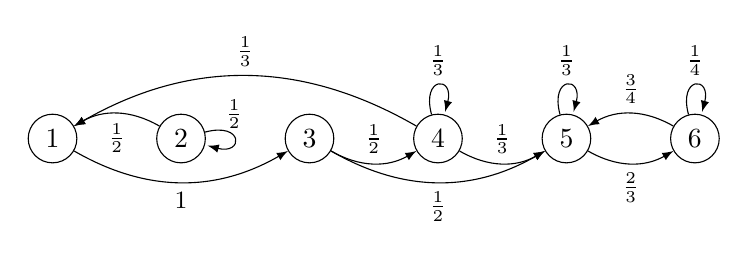
\begin{tikzpicture}[
              state/.style={
                  draw,
                  circle,
                  minimum size=1em,
                },
              every loop/.append style={-latex},
              start chain=going right
            ]
            \foreach \Value in {1,...,6}
            \node[state,on chain] (s\Value) {\Value};
            \path[-latex]
            (s1) edge[bend right] node[below,font=\small] {\(1\)} (s3)
            (s2) edge[bend right] node[below,swap,font=\small] {\(\frac{1}{2}\)} (s1)
            (s2) edge[loop right] node[above,swap,font=\small] {\(\frac{1}{2}\)} (s2)
            (s3) edge[bend right] node[above,swap,font=\small] {\(\frac{1}{2}\)} (s4)
            (s3) edge[bend right] node[auto,swap,font=\small] {\(\frac{1}{2}\)} (s5)
            (s4) edge[bend right] node[auto,swap,font=\small] {\(\frac{1}{3}\)} (s1)
            (s4) edge[loop above] node[above,swap,font=\small] {\(\frac{1}{3}\)} (s4)
            (s4) edge[bend right] node[above,swap,font=\small] {\(\frac{1}{3}\)} (s5)
            (s5) edge[loop above] node[above,swap,font=\small] {\(\frac{1}{3}\)} (s5)
            (s5) edge[bend right] node[auto,swap,font=\small] {\(\frac{2}{3}\)} (s6)
            (s6) edge[bend right] node[above,swap,font=\small] {\(\frac{3}{4}\)} (s5)
            (s6) edge[loop above] node[above,swap,font=\small] {\(\frac{1}{4}\)} (s6)
            ;
          \end{tikzpicture}
          \caption{State transition diagram for \(P_{1}\)}
          \label{fig:state-transition-diagram-p1}
        \end{answerfigure}
        From Figure~\ref{fig:state-transition-diagram-p1}, the communicating classes are
        \begin{empheq}[box=\fbox]{align*}
          \C_{1} &= \{1,3,4\} & &\text{which is transient} \\
          \C_{2} &= \{2\}     & &\text{which is transient} \\
          \C_{3} &= \{5,6\}   & &\text{which is recurrent}
        \end{empheq}
      \end{proofpart}

      \begin{proofpart}
        \((P_{2})\)

        \begin{answerfigure}
          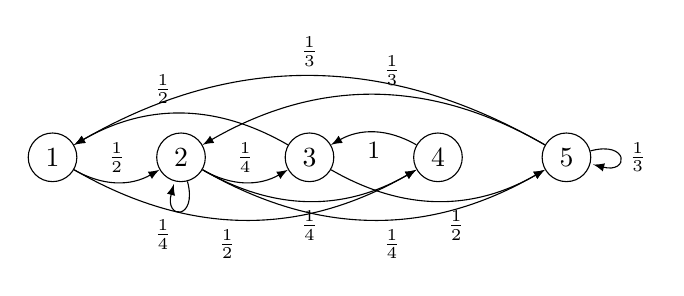
\begin{tikzpicture}[
              state/.style={
                  draw,
                  circle,
                  minimum size=1em,
                },
              every loop/.append style={-latex},
              start chain=going right
            ]
            \foreach \Value in {1,...,5}
            \node[state,on chain] (s\Value) {\Value};
            \path[-latex]
            (s1) edge[bend right] node[above,swap,font=\small] {\(\frac{1}{2}\)} (s2)
            (s1) edge[bend right] node[below left,swap,font=\small] {\(\frac{1}{2}\)} (s4)
            (s2) edge[loop below] node[below left,swap,font=\small] {\(\frac{1}{4}\)} (s2)
            (s2) edge[bend right] node[above,swap,font=\small] {\(\frac{1}{4}\)} (s3)
            (s2) edge[bend right] node[below,swap,font=\small] {\(\frac{1}{4}\)} (s4)
            (s2) edge[bend right] node[below right,swap,font=\small] {\(\frac{1}{4}\)} (s5)
            (s3) edge[bend right] node[above left,swap,font=\small] {\(\frac{1}{2}\)} (s1)
            (s3) edge[bend right] node[below right,swap,font=\small] {\(\frac{1}{2}\)} (s5)
            (s4) edge[bend right] node[below,swap,font=\small] {\(1\)} (s3)
            (s5) edge[bend right] node[above,swap,font=\small] {\(\frac{1}{3}\)} (s1)
            (s5) edge[bend right] node[above right,swap,font=\small] {\(\frac{1}{3}\)} (s2)
            (s5) edge[loop right] node[right,swap,font=\small] {\(\frac{1}{3}\)} (s5)
            ;
          \end{tikzpicture}
          \caption{State transition diagram for \(P_{2}\)}
          \label{fig:state-transition-diagram-p2}
        \end{answerfigure}
        From Figure~\ref{fig:state-transition-diagram-p2}, the single communicating class is
        \begin{empheq}[box=\fbox]{align*}
          \C_{1} &= \{1,2,3,4,5\}\quad & &\text{which is recurrent}
        \end{empheq}
      \end{proofpart}
    \end{solution}
  \end{questions}
\end{document}
